\documentclass[11px, a4paper, twocolumn]{article}

\usepackage[utf8]{inputenc}
\usepackage[swedish]{babel}

\usepackage{graphicx}
\usepackage{epstopdf}
\usepackage{color}
\usepackage[final]{pdfpages}
\usepackage{subfigure}
\usepackage{float}
\usepackage{caption}

\usepackage[hyphens]{url}
\usepackage[breaklinks,pdfpagelabels=false]{hyperref}

\usepackage{appendix}
\usepackage{tocvsec2}

\usepackage{biblatex}
%\usepackage{natbib}


%New Commands
\newcommand{\mail}[1]{\href{mailto:#1}{\nolinkurl{#1}}}


\bibliography{references}


\hypersetup{
    pdftitle={Picture Hunter},
    pdfauthor={Daniel Ström},
    colorlinks=true,
    citecolor=magenta,
    filecolor=magenta,
    linkcolor=black,
    urlcolor=magenta
}


\title{Picture Hunter}
\author{Daniel Ström \\ \mail{D@nielstrom.se}}

\begin{document}

\maketitle

\begin{abstract}
	Detta är en sammanfattning.
\end{abstract}

\tableofcontents

\listoffigures


\section{Koncept}
	Detta är det första avsnittet \cite{DesignGuidelines}. Detta är en länk: \url{http://developer.android.com/design/index.html}

    \begin{figure}
        \centering
        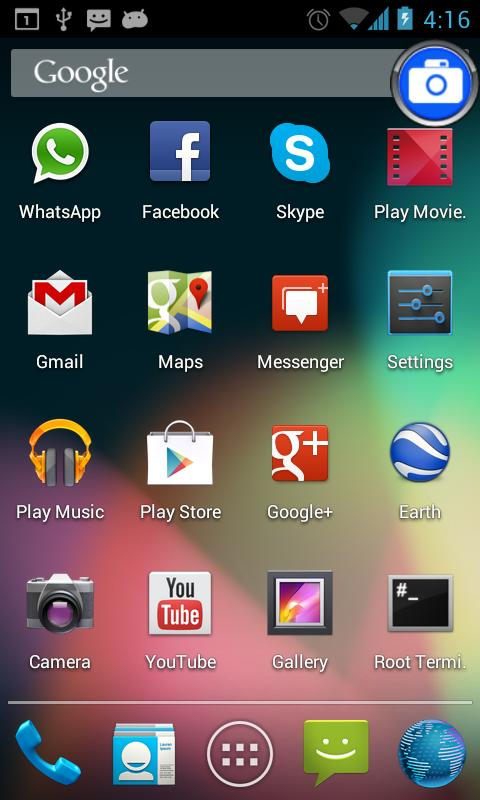
\includegraphics[width=\linewidth]{img/unnamed}
        \caption{\label{fig:android} A picture of an Android.}
    \end{figure}

    Detta är en referens till figur \ref{fig:android}.



\begingroup
\raggedright
\printbibliography
\addcontentsline{toc}{section}{Referenser}
\endgroup

\end{document}